\documentclass[10pt,a4paper]{article}
\usepackage[margin=19mm]{geometry}
\usepackage[T1]{fontenc}\usepackage{tgheros,textcomp}
\renewcommand{\familydefault}{\sfdefault}
\usepackage{xcolor,tikz,pgfplots,booktabs,hyperref,fancyhdr,array}
\usetikzlibrary{arrows.meta,positioning,calc,patterns}
\pgfplotsset{compat=1.18}
\definecolor{navy}{HTML}{171717}\definecolor{teal}{HTML}{242424}
\definecolor{gold}{HTML}{A0A0A0}\definecolor{pale}{HTML}{F2F2F2}\definecolor{muted}{HTML}{626262}
\hypersetup{colorlinks=true,urlcolor=teal,pdftitle={Aktina technical brief},pdfauthor={Loukas Louka; Aktina team}}
\pagestyle{fancy}\fancyhf{}\fancyhead[L]{\small\color{teal} AKTINA}
\fancyhead[R]{\small TEAM REVIEW DRAFT}\fancyfoot[R]{\small\thepage}
\fancyfoot[L]{\scriptsize Historical weather; illustrative plant}
\renewcommand{\headrulewidth}{.3pt}\setlength{\headheight}{15pt}
\setlength{\parindent}{0pt}\setlength{\parskip}{7pt}\color{navy}
\newcommand{\titleline}[2]{{\small\color{teal} #1}\par\vspace{3mm}{\fontsize{29}{33}\selectfont\bfseries #2}\par\vspace{4mm}}
\newcommand{\smallhead}[1]{\vspace{3mm}{\large\bfseries #1}\par}
\begin{document}
\titleline{SOLUTION}{Make water. Store it for later.}
Aktina tests whether a desalination unit and water tank can shift production toward available solar. Recovering electricity that would otherwise be curtailed requires spare plant capacity, usable storage and grid coordination. The demonstration does not measure that recovery.

\begin{center}
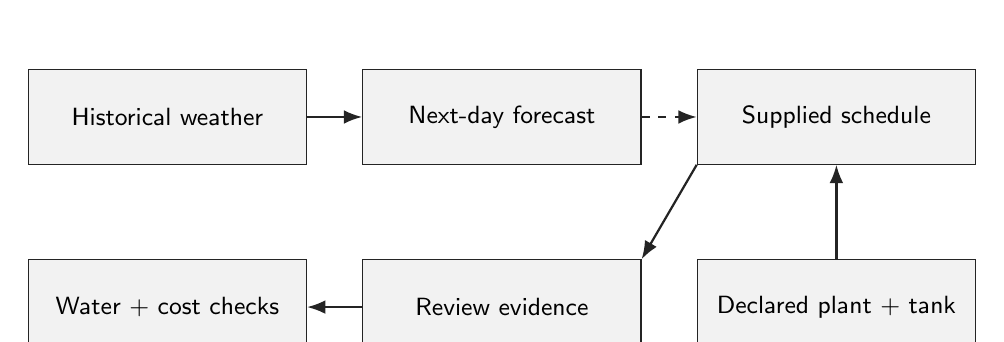
\begin{tikzpicture}[>=Latex,node distance=7mm,box/.style={draw=teal,fill=pale,align=center,text width=3.3cm,minimum height=1.2cm,font=\small}]
\node[box] (weather) {Historical weather};
\node[box,right=of weather] (forecast) {Next-day forecast};
\node[box,right=of forecast] (schedule) {Supplied schedule};
\node[box,below=12mm of schedule] (plant) {Declared plant + tank};
\node[box,left=of plant] (operator) {Review evidence};
\node[box,left=of operator] (water) {Water + cost checks};
\draw[->,thick,teal] (weather)--(forecast);
\draw[->,thick,teal,dashed] (forecast)--(schedule);
\draw[->,thick,teal] (plant)--(schedule);
\draw[->,thick,teal] (schedule.south west)--(operator.north east);
\draw[->,thick,teal] (operator)--(water);
\end{tikzpicture}
\par{\small\color{muted} Dashed link: the supplied schedule uses persistence, not the displayed LightGBM forecast.}
\end{center}

\smallhead{What runs now}
The demo loads Stefanos's retained files locally: 7,104 hourly schedule rows across 296 complete days, 6 December 2025--28 September 2026. It shows sun, production, tank inventory and illustrative cost. AktinaBench compares every retained validation and test prediction, plus six separate experiments. No model is fitted and no external API is called during the demo.

\begin{center}
\begin{tabular}{@{}ll@{}}\toprule
Supplied scheduler & Illustrative setting \\\midrule
Production range & $100$--$400\ \mathrm{m^3/h}$ \\
Demand & Hourly shape; summer and recorded-temperature factors \\
Tank / minimum & $4{,}000\ \mathrm{m^3}$ / $800\ \mathrm{m^3}$ \\
Starting stock & $2{,}000\ \mathrm{m^3}$ at each retained period's start \\
Specific electricity & $3.4\ \mathrm{kWh/m^3}$ \\
Price rule & \texteuro101/MWh if actual radiation $>600\ \mathrm{W/m^2}$; else \texteuro183 \\\bottomrule
\end{tabular}
\end{center}

\smallhead{Keep the water accounting visible}
\[
S_{h+1}=S_h+q_h-d_h.
\]
$S$ is stored water, $q$ hourly production and $d$ hourly demand. Stock carries between days within each period; the validation/test simulations restart separately. Equal daily ending stock is not enforced. Inspect production and stock change alongside cost: a cheaper day may draw down the tank. Hourly tank samples cannot establish between-hour or physical plant safety.

\smallhead{Which forecast made the plan?}
The supplied export is reproduced byte for byte by selecting persistence in the original scheduler. Running Stefanos's unchanged model-driven scheduler separately changes 469 production hours. Both outputs are retained; the website keeps the supplied export unchanged. Stefanos must confirm which schedule is intended for submission. Demand uses recorded target-day temperature, so this remains a retrospective scenario.

\newpage
\titleline{EVIDENCE}{Show the result and the control.}
3 July 2026: the supplied plan and flat production each make 5,658 m\textsuperscript{3}. The supplied tank starts and ends at 966 m\textsuperscript{3}. Shading marks actual radiation above 600 W/m\textsuperscript{2}, which triggers the illustrative discount; it is not a curtailment measurement.

\begin{center}
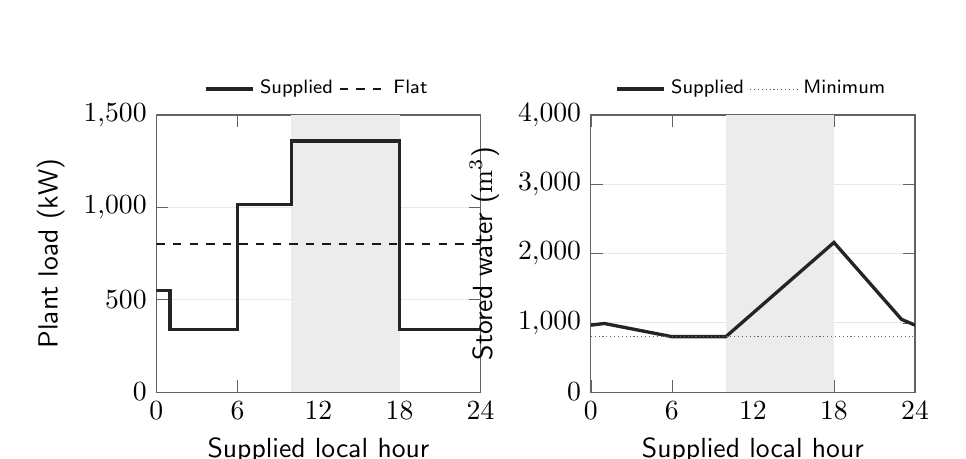
\begin{tikzpicture}
\begin{axis}[name=load,width=.47\linewidth,height=5.1cm,xmin=0,xmax=24,ymin=0,ymax=1500,
xtick={0,6,12,18,24},ylabel={Plant load (kW)},xlabel={Supplied local hour},
axis line style={muted},tick style={muted},ymajorgrids=true,grid style={muted!15},
legend style={draw=none,at={(.5,1.02)},anchor=south,legend columns=2,font=\scriptsize}]
\path[fill=muted!12] (axis cs:10,0) rectangle (axis cs:18,1500);
\addplot[const plot,teal,very thick] coordinates {(0,550.8)(1,340)(2,340)(3,340)(4,340)(5,340)(6,1016.6)(7,1016.6)(8,1016.6)(9,1016.6)(10,1360)(11,1360)(12,1360)(13,1360)(14,1360)(15,1360)(16,1360)(17,1360)(18,340)(19,340)(20,340)(21,340)(22,340)(23,340)(24,340)};
\addplot[navy,dashed,thick] coordinates {(0,801.55)(24,801.55)};
\legend{Supplied,Flat}
\end{axis}
\begin{axis}[at={(load.south east)},anchor=south west,xshift=14mm,width=.47\linewidth,height=5.1cm,xmin=0,xmax=24,ymin=0,ymax=4000,
xtick={0,6,12,18,24},ylabel={Stored water ($\mathrm{m^3}$)},xlabel={Supplied local hour},
axis line style={muted},tick style={muted},ymajorgrids=true,grid style={muted!15},
legend style={draw=none,at={(.5,1.02)},anchor=south,legend columns=2,font=\scriptsize}]
\path[fill=muted!12] (axis cs:10,0) rectangle (axis cs:18,4000);
\addplot[teal,very thick] coordinates {(0,966)(1,990)(2,952)(3,914)(4,876)(5,838)(6,800)(7,800)(8,800)(9,800)(10,800)(11,970)(12,1140)(13,1310)(14,1480)(15,1650)(16,1820)(17,1990)(18,2160)(19,1938)(20,1716)(21,1494)(22,1272)(23,1050)(24,966)};
\addplot[muted,densely dotted] coordinates {(0,800)(24,800)};
\legend{Supplied,Minimum}
\end{axis}
\end{tikzpicture}
\end{center}
Illustrative cost: \texteuro2,628.25 supplied versus \texteuro2,994.59 flat, a 12.23\% reduction. Both use 19,237.2 kWh. This establishes neither a model-specific gain nor recovered solar. The original model-driven scheduler reports unit-cost reductions of 3.6\% in winter--spring and 10.0\% in summer; persistence reports 3.6\% and 10.2\%.

\smallhead{Original forecast: full retained periods}
\begin{center}
\begin{tabular}{@{}llrrrr@{}}\toprule
Period & Method & MAE & Precision & Recall & F1 \\\midrule
Validation & LightGBM & 29.34 & .8142 & .7876 & .8007 \\
3,566 hours & Persistence & 32.47 & .7974 & .7974 & .7974 \\
Test & LightGBM & 14.27 & .9757 & .9554 & .9655 \\
3,567 hours & Persistence & 12.26 & .9801 & .9752 & .9777 \\\bottomrule
\end{tabular}
\par{\small\color{muted} MAE in W/m\textsuperscript{2}; positive label: actual radiation strictly above 600 W/m\textsuperscript{2}.}
\end{center}
The test model loses on all displayed measures. Validation informed early stopping; the two periods use different fitted models. The original adjacent splits lack a 24-hour boundary purge. All retained rows, including partial boundary days, remain in the benchmark.

\smallhead{Archived weather and residual corrections}
On the same 3,567 test hours, fixed archived weather forecasts reach MAE 8.81 W/m\textsuperscript{2}, precision .9851, recall .9832 and F1 .9841. Raw residual analogues reduce MAE to 6.92, but add one false alarm: 16 versus 15, with 17 misses for both. Validation retains the archived forecast. These retrospective results use a model-derived reference; historical publication times are unverified. No learned correction is promoted.

\newpage
\titleline{HANDOFF}{Keep ownership and evidence clear.}
\smallhead{Roles}
\begin{center}
\begin{tabular}{@{}>{\raggedright\arraybackslash}p{.26\linewidth}>{\raggedright\arraybackslash}p{.67\linewidth}@{}}\toprule
Stefanos & Original LightGBM model, plant assumptions, scheduler and roadmap. Confirm the intended schedule and next model version. \\
Loukas Louka & Original concept; application, integration, evaluation and separate improvement experiments. Original model files remain unchanged. \\
Andreas Nikolaides / Cleopas Cleopa & Business case and pitch. No technical model ownership assigned. \\\bottomrule
\end{tabular}
\end{center}

\smallhead{Demo and backup}
Open \href{https://aktina-pafos-2026.vercel.app}{Aktina}, then choose 3 July, 10 December and 16 March. Inspect sun, supplied production and ending tank stock before cost. On 16 March the model's MAE is 48.48 versus 156.33 W/m\textsuperscript{2} for persistence; this selected day does not replace the full test. Open \href{https://aktina-pafos-2026.vercel.app/benchmark.html}{AktinaBench} for both periods and every candidate.

The packaged site needs no internet. \texttt{Aktina-Backup-Final.mp4} is a silent 44-second screenshot walkthrough, not a live interaction recording. Two team rehearsals remain.

\smallhead{Next model evidence}
Solar geometry, fixed archived forecasts and historical residual scenarios have been tested separately from the original model. Against satellite estimates on 3,517 common test hours, archived-forecast F1 is .9659 and raw-analogue F1 is .9654; 50 missing hours remain unscored. Satellite estimates are not ground sensors. Future forecasts are locked for a separate later check; competition delivery uses the completed evidence. No v2 gain is established.

\smallhead{Pilot and business scope}
Grid needs operator-confirmed demand, plant limits, meter data, tariffs and usable curtailment signals. Pressure, flushing, water quality, ramps and maintenance remain outside the supplied scheduler. Sites remains a separate garden/leak prototype; its synthetic checks are not field validation. Pricing, customer agreements and savings are unverified.

\smallhead{Submission checks}
Confirm the intended schedule with Stefanos, reconcile the slides with this evidence, and rehearse the offline demo. Confirm the team contact and required declarations before submission. Do not present the earlier reference experiment as Stefanos's model.

\vfill
\hrule height .5pt\vspace{3mm}
{\footnotesize Evidence, 4 October 2026: \href{https://github.com/stefanosbordea/actina/tree/stefanos-model}{Stefanos's repository}, model source at \texttt{2a093ab}.\par
Retained checks: \texttt{app/handoff/ACTINABENCH.md}, \texttt{scheduler-reproduction/README.md}, \texttt{MODEL-V2-FEEDBACK.md}; research results: \texttt{app/experiments/README.md}.\par
Historical Open-Meteo weather; source labels use a recovered fixed UTC+03 clock. The scheduler has already shifted prediction-origin timestamps by 24 hours; the demo does not shift them again. No plant operating authority is claimed.}
\end{document}
